\chapter{Conclusion}
\minitoc
\section{Recap}
The goal of this thesis was to explore the ability of different types of GIRG model to match real social network graphs with some suspected inherent geometry and power law degree distribution. In documenting our various experiments, we also detail our methods and ideas for working with GIRGs and graph data which may prove useful to other practitioners.

Our first effort was to follow the realism framework of \cite{blasius2018towards}, to compare a range of generative graph models, including many GIRG subtypes, in their ability to replicate global statistics of a set of $\sim 100$ social network graphs.
With this framework we did find GIRGs able to outperform on a few statistics: closeness centrality, betweenness centrality, effective diameter, and mean local clustering coefficient. We identified differences between different GIRG variants, with max cube GIRGs excelling at diameter replication, MCD GIRGs on closeness centrality, and max torus GIRGs on betweenness centrality. Not much difference was found by increasing the geometric dimension, suggesting that 1-3 dimensions may be sufficient for high level similarity to real graphs, and indeed 1d is often the best.

We then explored fitting GIRG node geometric location parameters to the real graphs, to see if GIRGs are capable of exact replication on a node and edge level. This proved quite successful, showing that GIRGs can capture a high percentage of edges, even with just 1 dimension. Adding further dimensions is computationally intensive and doesn't increase the fit substantially. Our range of fitting methods might be further refined in practice according to the use case. 

Future work might investigate more into how 1 dimensional geometry already fits the data quite well, in particular seeing if the variants of distorted GIRGs or min/max mixed GIRGs can explain a relative ordering of dimension importance. Intuitively 1 dimension may be the most influential for our social connections, but surely our friendships are more multifaceted.


\paragraph{Thanks} to my supervisors Marc Kaufmann and Ulysse Schaller, as well as Johannes Lengler, for their valuable input and guidance throughout the thesis. Many thanks to Angelika Steger and her lab for their friendly and welcoming research environment. Finally much appreciation to friends, family, ETH, etc. for their support and existence. And thanks to the reader for making it this far! I hope it's been an enjoyable/interesting reading experience.




% \begin{figure}
%   \centering
% 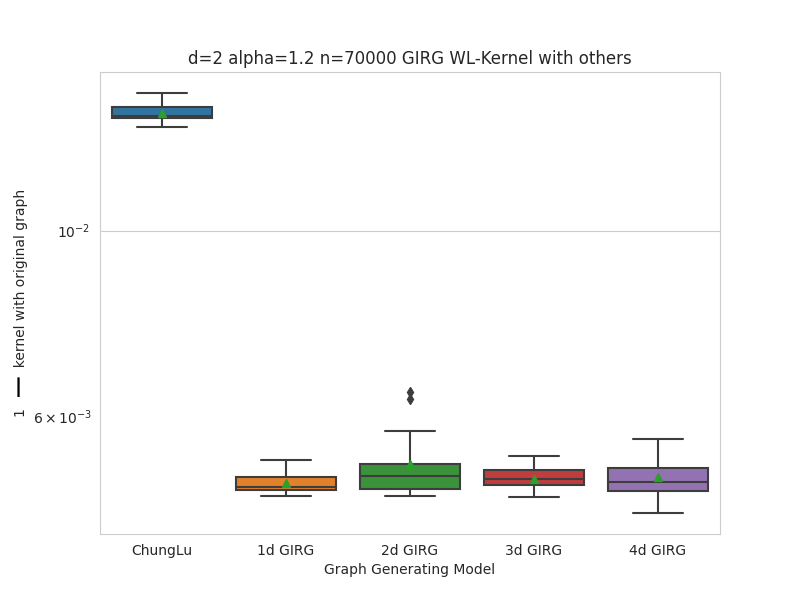
\includegraphics[width=0.8\linewidth]{figures/d=2 alpha=1.2 n=70000 GIRG WL-Kernel with others.png}
% \caption{WL-Kernel of a d=2, alpha=1.2, n=70000 Torus GIRG with other generated graphs (13 per model). All the GIRGs are more similar to the original than Chung-Lu, but we cannot differentiate between different GIRGs.}
% \label{fig:wl_kernel_gentorus}
% \end{figure}

% socfb-Brandeis99 d=3.png


% \begin{figure}
%   \centering
% 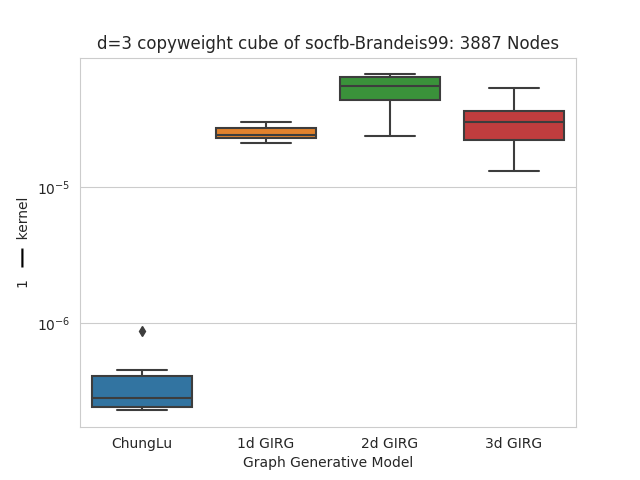
\includegraphics[width=0.8\linewidth]{figures/socfb-Brandeis99 d=3.png}
% \caption{RW-Kernel of a d=3 copy weight cube GIRG fit to socfb-Brandeis99 (matching number of edges and local clustering coefficient), with other generated graphs (6 per model type). Chung-Lu graphs have highest similarity to the original, despite it being a 3D GIRG}
% \label{fig:rw_kernel_fitcopycube}
% \end{figure}


